%%%%%%%%%%%%%%%%%%%%%%%%%%%%%%%%%%%%%%%%%%%%%%%%%%%%%%%%%%%%%%%%%%%%%%%%%%%%%%%%
%2345678901234567890123456789012345678901234567890123456789012345678901234567890
%        1         2         3         4         5         6         7         8

\documentclass[letterpaper, 10 pt, conference]{ieeeconf}  % Comment this line out
                                                          % if you need a4paper
%\documentclass[a4paper, 10pt, conference]{ieeeconf}      % Use this line for a4
                                                          % paper

\IEEEoverridecommandlockouts                              % This command is only
                                                          % needed if you want to
                                                          % use the \thanks command
\overrideIEEEmargins
% See the \addtolength command later in the file to balance the column lengths
% on the last page of the document



% The following packages can be found on http:\\www.ctan.org
%\usepackage{graphics} % for pdf, bitmapped graphics files
%\usepackage{epsfig} % for postscript graphics files
%\usepackage{mathptmx} % assumes new font selection scheme installed
%\usepackage{times} % assumes new font selection scheme installed
%\usepackage{amsmath} % assumes amsmath package installed
%\usepackage{amssymb}  % assumes amsmath package installed

\title{\LARGE \bf
Light-Fidelity - Electromagnetic data transmission using visible light
}

% \author{ \parbox{3 in}{\centering Huibert Kwakernaak*
%         \thanks{*Use the $\backslash$thanks command to put information here}\\
%         Faculty of Electrical Engineering, Mathematics and Computer Science\\
%         University of Twente\\
%         7500 AE Enschede, The Netherlands\\
%         {\tt\small h.kwakernaak@autsubmit.com}}
%         \hspace*{ 0.5 in}
%         \parbox{3 in}{ \centering Pradeep Misra**
%         \thanks{**The footnote marks may be inserted manually}\\
%        Department of Electrical Engineering \\
%         Wright State University\\
%         Dayton, OH 45435, USA\\
%         {\tt\small pmisra@cs.wright.edu}}
% }

\author{ \parbox{3 in}{\centering Man-Leong Chan
        School of Electronic and Computer Science\\
        University of Southampton\\
        {\tt\small mlc1g14@ecs.soton.ac.uk}}
}

\usepackage{graphicx}
\usepackage{booktabs}
\usepackage{siunitx}
\usepackage{mathtools}
\DeclarePairedDelimiter\ceil{\lceil}{\rceil}
\DeclarePairedDelimiter\floor{\lfloor}{\rfloor}
\usepackage{pifont}

\begin{document}



\maketitle
\thispagestyle{empty}
\pagestyle{empty}


%%%%%%%%%%%%%%%%%%%%%%%%%%%%%%%%%%%%%%%%%%%%%%%%%%%%%%%%%%%%%%%%%%%%%%%%%%%%%%%%
\begin{abstract}

Lifi has amazed the industry in terms of its high-speed performance and its subtleness of its application. However the industry remains skeptical on the possibility of it being a real applicable technology in the near future. In order to investigate the technological challenges that Lifi is facing, we tried to implement the very basic version of a Lifi system.\\ \\
The goal of this project is to successfully transmit a set of ASCII characters from the transmitter to the receiver using Lifi. This project will cover some aspect of physical (L1) and data link (L2) layer of the OSI model, aiming to achieve a simple unidirectional communication, limited by time and cost. 

\end{abstract}
%%%%%%%%%%%%%%%%%%%%%%%%%%%%%%%%%%%%%%%%%%%%%%%%%%%%%%%%%%%%%%%%%%%%%%%%%%%%%%%%
\section{INTRODUCTION}

Lifi or Light-Fidelity is a high-speed network communication technology using visible light. While Lifi and WiFi both transmit data electromagnetically, Lifi is able to achieve a much higher theoretical bandwidth due to the high frequency of visible light in Lifi compared to a lower frequency of radio waves used by WiFi.
While researchers at University of Oxford had been able to achieve a staggering 224 Gb/s \cite{Gomez2015a}, the goal of this project is to investigate the basis of transmitting data through air using visible light at a low cost. 
\\ \\
In the physical layer, we experimented with ways to transmit simple binary signal from one end to another in order to determine the hardware that is required. In the data link layer, we explored methods to convert binary to ASCII and vise versa in real time, as well as a methodology for error handling. All together it allowed us to define a simple networking protocol suitable for low-powered unidirectional communication. 

\section{Physical Layer}

Both the transmitter and the receiver is based on a programmable single-board computer NXP FRDM-K64F \cite{NXP2014} with 120MHz processor and 1 MB of flash memory. The transmitter sends data by driving a green LED using a 3.3V GPIO pin \textit{(Fig. 1)}, while the receiver is connected to a TEPT5700 Ambient Light Sensor\cite{VISHAY} (photodiode) which is most sensitive to the green light region.
\\ \\
Transmission speed is limited by the clock rate of the K64F board which can only drive the LED signal or the photodiode at a lower speed. The lack of power provided by the GPIO pins also contributed to the lower speed as the LED will not be as bright compared to a higher voltage output. This increase the photodiode's challenge to detect clear signal, therefore likely to create more signaling or interpretation error. 

\begin{figure}[h!]
  \centering
  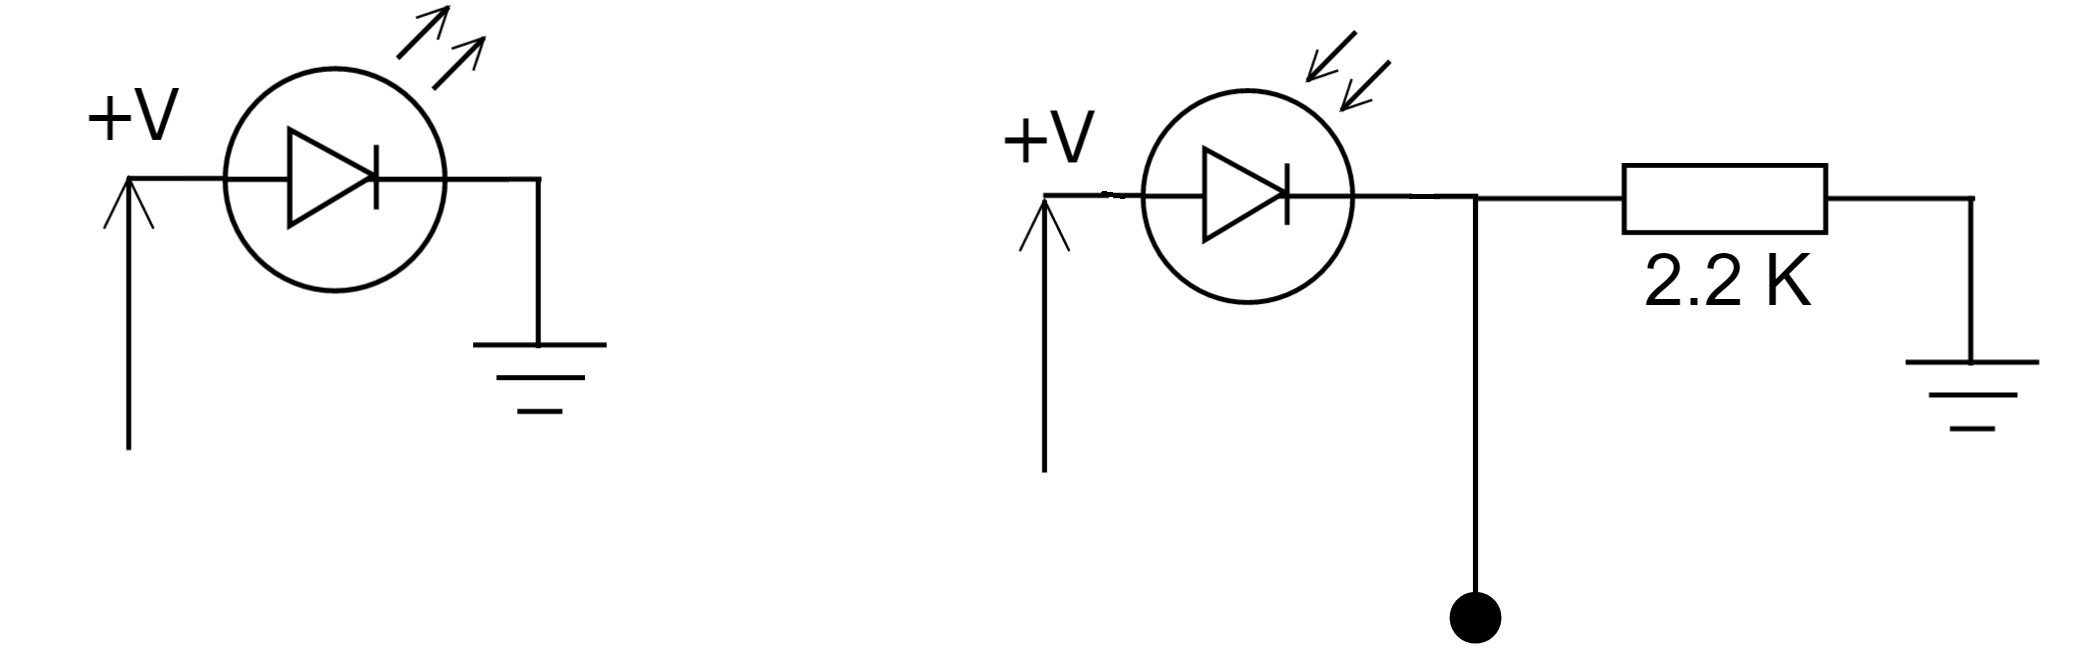
\includegraphics[width=0.4\textwidth]{circuit.png}
  \caption{Circuitry of the transmitter (left) and receiver (right)}
\end{figure}

\subsection{Sensing}

A popular Lifi implementation in the industry is to utilize all the indoor lighting such that it provides a stable single source of signal in the form of visible light. In this project however it is not viable for us to find indoor light sources capable of oscillating at a high frequency. Instead we have uses an LED as the source and photodiode as the sensor. 
\\ \\
The LED is connected to a 3.3V GPIO digital-out, at this level of voltage the LED does not glow very bright compared to the lab’s background light. Therefore we have to enclose the area between the LED and the photodiode in order to minimize the interference. To further enhance the signal level, the colour of LED is carefully chose according to the peak sensitivity of our TEPT5700 Ambient Light Sensor\cite{VISHAY} at 560 nm which is a lime-green colour. 


\subsection{Performance}

While the performance of the transmitter and receiver is not part of the project scope, it is crucial for investigating a viable transmission frequency. The maximum theoretical throughput of the transmission is limited by the poorest performing hardware in the entire system, it would also define the operating speed between both ends. Therefore both transmitter and the receiver has undergone performance testing measure using a high-performance oscilloscope. 
\\ \\
The transmitter with an LED is driven by a 120MHz processor. It has a maximum driving speed of 794.9 KHz turning an LED on and off, however the performance was dramatically reduced when it has to process data along with transmission. 

\begin{figure}[h!]
  \centering
  \begin{tabular}{lll} \toprule
   & Frequency & Period\\ \midrule
  Binary Pair & 794.9\SI{}{\kilo\hertz} & 1.258\SI{}{\micro\second} \\
  Mean & 794.7\SI{}{\kilo\hertz} & 1.258\SI{}{\micro\second} \\
  Minimum & 795.3\SI{}{\kilo\hertz} & 1.257\SI{}{\micro\second} \\
  Maximum & 152.9\SI{}{\kilo\hertz} & 1.259\SI{}{\micro\second} \\
  Std-Dev & 152.9\SI{}{\hertz} & 242.2\SI{}{\pico\second} \\ \bottomrule
  \end{tabular}
  \caption{Signal frequency and period tested using an oscilloscope}
\end{figure}

\section{Digital Modulation}
\subsection{ADC}

Our system relies on On-Off keying to transmit data from transmitter to receiver. It uses unipolar encoding where an LED at full brightness represent \textit{one} and off  representing \textit{zero}. Other implementation where zeros are represented half the brightness of representation of ones is unsuitable, as brightness is measured relative to the surrounding environment. If the photodiode is to determine the exact brightness transmitted from the LED, the distance between both transmitter and receiver must be kept constant\cite{JoshuaE.Barnes2003}. Such implementation would require very accurate laboratory set up and limits the mobility of the entire system.
\\ \\
When the transmitter is sending unambiguous binary signals, the photodiode receiver will receive an analog value between 0-255 according to the level of brightness it detects. This requires an analog-to-digital(ADC) module to determine whether the LED has transmitted \textit{one} or \textit{zero}. In our implementation, we have determined a threshold such that any value above the threshold will represent \textit{one} and any below would represent \textit{zero}. Such threshold is not a fix value and is determined before any signal is sent. Depending on the surrounding background brightness, the threshold is increase if the background brightness is high or decrease if the brightness is low. 


\subsection{Binary Encoding}
We have discussed the benefit of unipolar encoding above, however leaves ambiguity between \textit{zero} when the LED is off and when no signal is being sent. Therefore the receiver will not be able to differentiate between '0110' and '110', as the '0' in the first string is represented by no light emitted from the LED. 
\\ \\ 
In order to tackle this problem, we have employed a binary encoding to represent \textit{one}s \& \textit{zero}s. Instead of having LED on \& off representing the values directly, we encode \textit{one}s \& \textit{zero}s with on/off patterns.

\begin{figure}[h!]
  \centering
  \begin{tabular}{ll} \toprule
  On-Off Pattern & Binary \\ \midrule
  \textbf{ON}-OFF-OFF & 0 \\
  OFF-OFF-\textbf{ON} & 1 \\ \bottomrule
  \end{tabular}
  \caption{Signal frequency and period tested using an oscilloscope}
\end{figure}

If we use dot-and-dashes with '\ding{108}' representing the LED being on and '\_' LED off, we could demonstrate how the binary encoding would avoid ambiguity creating by unipolar encoding. Again with the same pair of string: '0110' \& '110'

\begin{figure}[h!]
  \centering
  \begin{tabular}{ll} \toprule
  Data & Encoded data \\ \midrule
  0110 &  \ding{108} \_ \_ \_ \_ \ding{108} \_ \_ \ding{108} \ding{108} \_ \_ \\
  110 & \_ \_ \ding{108} \_ \_ \ding{108} \ding{108} \_ \_ \\ \bottomrule
  \end{tabular}
  \caption{Signal frequency and period tested using an oscilloscope}
\end{figure}



\section{Data-Link Layer}

\subsection{Error Handling}
In many bidirectional communication, error is detected by the client and resolved by sending positive or negative acknowledgements. In a unidirectional communication however, the transmitter have no idea whether the signal is received by the receiver or if the packet content is valid. Therefore a good forward error correction (FEC) technique is important such that if the receiver happens to have receive the data, it can validate and possibly recover the content automatically. \cite{Clark1981}
\\ \\
There are many factors to consider when choosing a forward error correction technique:
\\
\subsubsection*{\textbf{Nature of most error}} 
Most error occur due to sensor’s thread halt, this occur when the sensor’s CPU get occupied and stop sensing data for a short period of time. If the halt time is short, FEC with interleaving would help recover the lost bits. 
\\
\subsubsection*{\textbf{Frequency of the error}}
Halt happens periodically but the period is unknown. Therefore a simple parity bit technique may not be sufficient to detect, never mind correct the error. The error detection ratio is highly important in case the error rate is high.
\\
\subsubsection*{\textbf{Real-timeness of the data output}}
We try to achieve real-time data receiving on the sensor side and therefore error correction will need to be handled as the binary data comes in. Therefore the length of the FEC message length should be as short as possible. A short FEC message allow us to process and correct data as soon as possible instead of queuing up a long FEC message.
\\
\subsubsection*{\textbf{Throughput}}
The ultimate throughput is not our consideration, so we have been very generous on error-correction-bit to data ratio
\\


\subsection*{Result}
Binary repetition code\cite{Bossert1999} is one of the best and simple solution for FEC over a binary erasure channel. It has a hamming distance of \textbf{n}, and an error correcting capacity of
\begin{equation*}
    \floor*{\frac{n - 1}{2}}
\end{equation*}
In the case of this project, we have allow extra redundancy with repetition code length of 21, which is equivalent to a (21,10) hamming code. This level of redundancy allow us to tolerate sampling error that may occur. Binary repetition code does not rely on interleaving, this allow us to process the data straight away for real-time output. Therefore there is very minimal data which is stored while the receiver is listening to the incoming signals.



\section{Encoding \& Decoding}

We have discussed the methodology of techniques we have used, now it is time to put together the workflow for both transmitter and receiver.

\subsection{Transmitter}

Encoding the signal is rather straight forward as we assume the data for transmission is fully given to the transmitter before the encoding begins. 

\begin{figure}[h!]
  \centering
  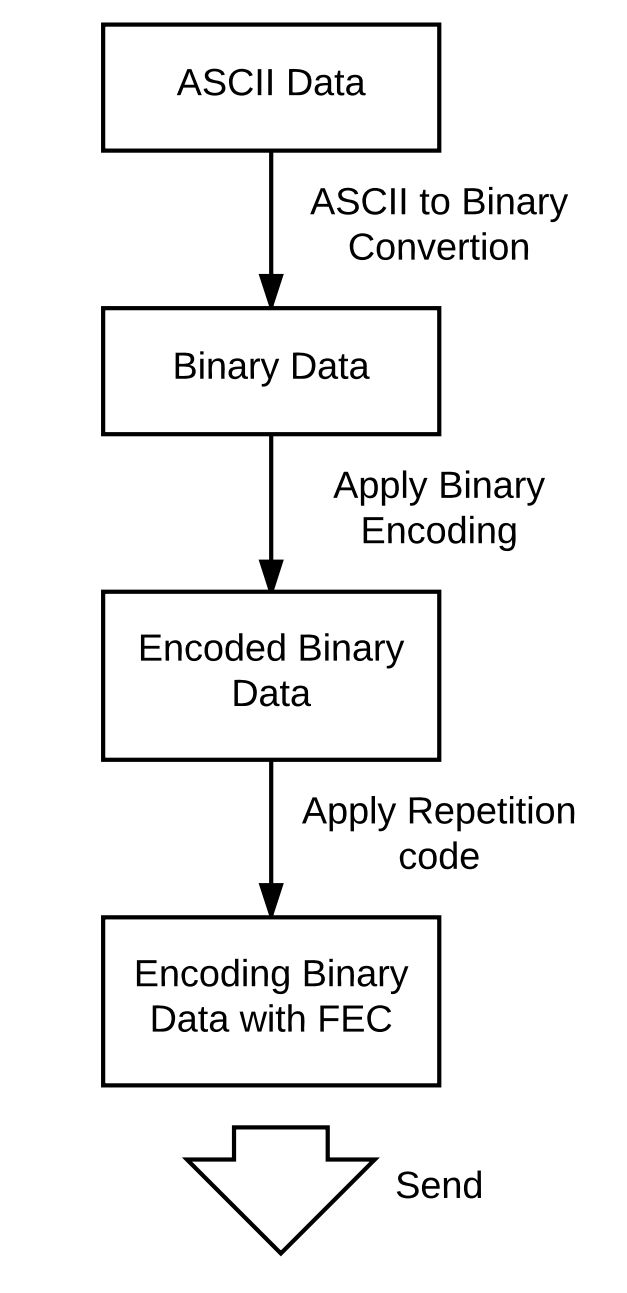
\includegraphics[width=0.2\textwidth]{Encode.png}
  \caption{Work flow for encoding ASCII character set}
\end{figure}

It starts with ASCII characters encoded into 7-bits binary data (Fig. 5). Binary encoding is then applied to every bit in the binary data, where \textit{zero} is encoded into '100' \& \textit{one} into '001'. Lastly FEC repetition code is applied where every encoded binary data is repeated 21 times before the encoded binary data with FEC is sent over the network.


\subsection{Receiver}

Decoding receiver's information is a little more complicated compared to transmitter as data can arrive at anytime. To make the task more complicated, receiver tries to decode the information as soon as they arrive such that it can minimize the data stored. 

\begin{figure}[h!]
  \centering
  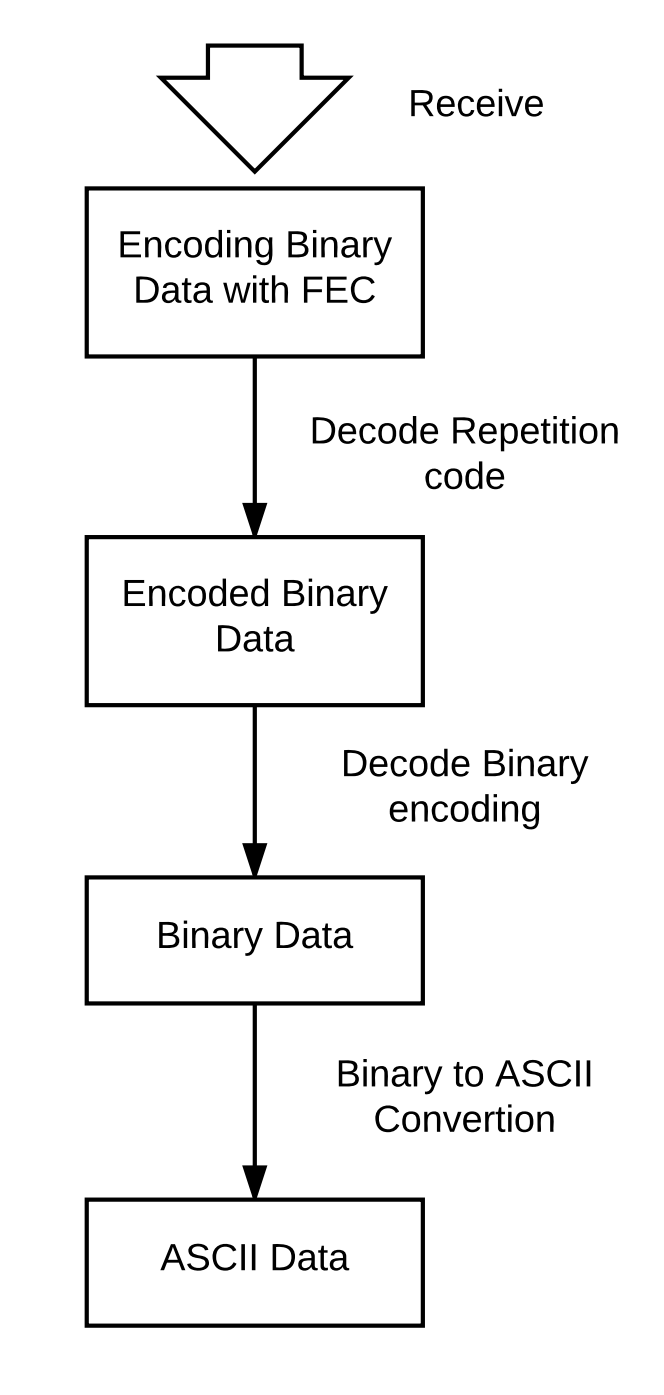
\includegraphics[width=0.22\textwidth]{Decode.png}
  \caption{Work flow for decoding incoming binary data}
\end{figure}

The receiver start by decoding repetition code (Fig. 6), the benefit of such FEC code is that it can be decode by calculating the statistical mode of the received bits according to the length of the repetition code. 
\\ \\
The receiver than has to decode the binary data. Which is a simple pattern matching process for every set of three bits and map '100' \& '001' to \textit{zero} \& \textit{one} respectively. E.g the encoded string '001100' would produce the binary '01'. When there is an error occurring in the data, the unrecognized data would be thrown away. For example the string '010100', the pointer will point at the first 3 bits '010' which is unrecognized, the first bit '0' will then be thrown away leaving the string '10100'. The process repeats again as the 3 bit string '010' is again unrecognizable. The same happens for the next bit leaving the string '100' left. The string now is recognizable and will be decoded into '0' in binary.
\\ \\
Finally, translating the decoded binary data into 7-bit ASCII very straight forward.




\section{Remaining Work}

The biggest challenge in unidirectional communication is clock synchronization. A synchronized clock between the sender and the receiver allows the signal to be interpolated at the correct time. Without the correct synchronization, the sender and receiver pair will soon be interpolating data at a different rate and producing error due to time drift. This is a common problem across all networking hardware and expensive time synchronization device are integrated into high-speed networking solutions.
\\ \\
In our implementation there is currently no time synchronization method applied to either of the device. We rely on frequent resetting of both device and the benefit of having 2 of the same hardware on the sender and the receiver side, because both device has the same CPU and clock rate, the time drift problem could be contained for a limited amount of time.
\\ \\
To make matter worst, unidirectional communication does not allow our receiver to give any time drift feedback. Therefore if the receiver does detect the effect of time drift, there is no possible way of notifying the sender on updating the time delta between them. The only possible way to achieve a certain level of clock sync without using external clock-sync device or bidirectional communication is to create another unidirectional communication. This extra unidirectional communication could send the clock of the transmitter by sending the clock rate of itself at the same time, a signal that sent the highest oscillation rate driven by the transmitter's CPU. This way the receiver would be able to tell the rate of the transmitter at any given time. 

\section{Conclusion}

Throughout this project, we have demonstrated many techniques on how to reliably transmit simple ASCII characters 'over the air'. It shows how difficult it could be to simply transfer data even at a lower rate using visible light. As mentioned in my remaining work, this project is by no means a household Lifi product ready to be deployed. However the project does give some indication on the challenges that we face in networking technologies of this nature. 


\section*{ACKNOWLEDGMENT}

I would like to thank my partner Devashish Dixit on his contribution and motivation at all stages of the project, as well as Prof Kirk Martinez \& Graeme Bragg for their guidance in this project.

\bibliographystyle{plain}
\bibliography{lifi.bib}

\end{document}
